\documentclass[]{article}

\usepackage{subcaption}
\usepackage{amssymb,amsmath,amsthm}
\usepackage{svg}
\usepackage{caption, subcaption}
\usepackage[backend=bibtex]{biblatex}  
\usepackage{todonotes}
\usepackage{graphicx}
\usepackage{hyperref}
\usepackage{etoolbox}

\graphicspath{ {./images/} }

\title{Literature Review on Cell tracking across videos from different points of view}
\author{Chrysostomos Chadjiminas}


\addbibresource{biblio.bib} 
\AtEndDocument{
	\clearpage
	\printbibliography
}

\begin{document}

\maketitle

\begin{abstract}
	This is a sample content
\end{abstract}


\section{Problem statement}

%\subsection{Apo to de Castro}

%A number of methods are available for measuring blood velocity. To date techniques that are based on Doppler velocimetry velocimetry [3, 4] including variations based on Optical Coherence Tomography (OCT) [5, 6] have been improved and demonstrated by many groups and have been most useful for relatively large retinal vessels (> 50 microns). Also blood flow can be related to the modulation of the speckle signal [7] but this technique tends to be useful only for large vessels as well. Direct imaging techniques have typically used 
%
%either dye injection [8–12] or externally labeled leukocytes re-injected into the blood stream [12, 13]. Currently Adaptive Optics techniques (AO) are able to provide higher resolution images of flow in small vessels without the need of contrast agents. Using an Adaptive Optics confocal Scanning Laser Ophthalmoscope (AOSLO) the velocity and pulsatility of the large moving features thought to be leukocytes [14], that can be observed moving through the capillaries of the macular region was determined either from the change in position of two consecutive frames of a video [14, 15] or from the change of intensity in a spatiotemporal plot [16, 17]. Also, AO has allowed the measurement of the erythrocyte velocities in small retinal regions either by using high frame rate non-confocal imaging [18], or by shrinking temporarily the field of view to a single scan line [19].
%Recently the use of an AOSLO with multiply scattered light detection [20, 21] has allowed improved imaging of the vasculature of the human retina. With this technique rbcs can be directly imaged while travelling through the capillaries of the human eye [22, 23]. The determination of rbcs velocity is desirable since they should provide a better estimate of tissue perfusion and vascular autoregulation than leukocytes, which are much larger than the capillary lumen and thus travel at a different velocity. While the single file flow of rbcs through capillaries simplifies velocity measures, their abundance introduces the issue of velocity aliasing for low frame rate systems, since the same cell cannot be identified between two consecutive frames. To solve this problem we developed a dual-channel AOSLO to image the retina with two close but different wavelengths. By introducing small angular shifts between the beams at the pupil, the same area of the retina is sampled at different times and this produces temporal offsets much smaller than the frame rate of the raster scan itself. Figure 1 shows the general principle of the approach. In the current study we introduced a separation of about 4.7 ms between channels and measured the change in position of the red blood cells during this interval to calculate velocity. Because the signal to noise ratio in our images is relatively low we calculated the average velocity over a 10 ms window and along a capillary segment.

%\subsection{Bedggood}
% Mapping flow velocity in the human retinal capillary network Cited by 2

%The retina is unique in that it affords direct, non-invasive observation of neural tissue and its associated vascular beds. 
%Recent developments in technology have made possible the visualization of the smallest vessels in the living human retina [1–4]. The smallest vessels within neural tissue offer the greatest resistance to flow and are thought to play a key role in mediating functional changes in flow [5, 6].
%
% Such vessels have been implicated early in the disease process for a variety of conditions including diabetes [7], hypertension [8], stroke [9] and dementia [10]. Recent studies of retinal capillaries using adaptive optics imaging suggest that overt structural damage to capillaries and larger vessels may be preceded by altered capillary flow patterns [11, 12]. Proper characterisation of microvascular flow in the retina may therefore prove important to help elucidate the course of progression for a range of important diseases, and to provide a more sensitive biomarker for the evaluation of potential treatments. Whilst it is now possible to observe individual blood constituents in the smallest retinal vessels [4], including erythrocytes, leukocytes and even platelets [13], quantifying rate of flow remains challenging due to their small size, low contrast, and high velocity relative to vessel
%
%
%diameter. Existing approaches include manual or part-manual labelling of data [13–15], which are time consuming and may not be amenable to assessment of large numbers of patients in clinical settings. It is possible to “freeze” the raster of a scanning system to rapidly image a given point on a vessel, as long as eye movements are tracked and compensated [13, 16]. This produces highly precise measurements of velocity and other rheological parameters at that position, at the expense of simultaneous collection of data across the vascular network. This paper will focus on automated approaches to determine velocity, from large numbers of vessels imaged simultaneously in a single video sequence. Previously advocated approaches applicable to this task include particle image velocimetry (“PIV” [4]) and the spatiotemporal kymograph (“STK” [17–21]), which suffer from various limitations summarised below. PIV involves the division of each spatially-registered image frame into small sub-regions. For each sub-region, the 2D cross-correlation between successive frames is calculated independently. The displacement of the peak of the cross-correlation indicates the distance that blood is presumed to have travelled between frames in a given sub-region. Inherent limitations include:

%\subsection{Apo ton Adam Dubis}
%​The purpose of tracking blood cells is to measure their speed, that is the obvious point. In actuality, we do not know the full effect of blood pressure on single cell blood flow, that is one of the points we want to look at. Why do we want to do this? In short everytime the heart beats, a bolus of blood leaves the heart at high pressure and speed and leaves into the vascular system of the body. The blood vessels, especially the vessels attached to leaving the heart (arteries) are elastic and are able to absorb this high pressure bolus and damped the pressure as the blood gets away from the heart and into the tissues (eye for us). Physiologically the goal of the smallest blood vessels is to facilitate the exchange of O2 out of the vessels and waste products CO2 out of the tissue. From a fluid dynamics standpoint this works best if there is a constant and consistent flow of blood at a single speed. As I mentioned the arteries, when young and healthy dampen the heart beat pressure wave into a near constant flow in the retinal tissue. As the vascular system ages, or damage is done to the vascular system (diabetes, heart disease, chronic inflammatory diseases), the arterial blood vessels are not able to dampen the rate of flow and so the pressure wave tracks down the blood vessel and into the capillaries. This changes occurs long before detectable disease occurs and to some extent is likely reversible. It is believed that this loss of vessel pulse dampening is responsible the the disease effects of diabetes, dementia, Parkinson's and Multiple Sclerosis. However there is no way to study this in the brain. The vascular system of the eye and brain are similar to each other and different from everywhere else in the body. Therefore we want to study the eye. I have put two papers one by deCastro et al and one by Bedggood et al that lay out this rationale in more depth.

%) Conclusions - We have treatments for MS and diabetes that we can apply that slow progression, but we need a biomarker that shows early progression. We hope that this imaging provides. The difference between what you said is that this imaging will not provide a treatment, it hopes to enable earlier treatment with existing interventions 

\subsection{Introduction}

In this thesis the main goal is to track and measure red blood cell velocity across frames captured within the eye retina.	
The images captured using an Adaptive Optics Light Scanning Opthalmoscope that was developed by my supervisor and him team.
From having videos of the red blood cell movement, one can deduce the velocity of the blood flow, among other characteristics.
By detecting the cells across frames, because the video is captured at a known fixed rate and the field of view is known, one can then extract the velocity of each red blood cell which is important for measuring the blood flow.

% Παράφραση from the Adam Dubis email
The retina is unique because, with development in adaptive optics, it allows for a non-invasive imaging of the vascular plexus inside the retina \cite{tam_noninvasive_2010}.
As the vascular system gets older, or damage is done to it from diabetes, heart disease, chronic inflammatory diseases or other neurological diseases, the arterial blood vessels are not able to dampen the rate of blood flow. As a result, the pressure wave tracks down the blood vessel and into the capillaries. 
These changes occur before the disease is detected. 
Contrary to the symptoms these diseases have at a later stage, these changes can be potentially reversed, effectively preventing the disease from causing more damage.  \todo{search for citations}
It is believed that this loss of vessel pulse dampening is responsible the disease effects of diabetes \cite{mizutani_accelerated_diabetes_1996}, dementia \cite{de_la_torre_is_alzheimer_2004}, stroke \cite{ostergaard_role_stroke_2013}, hypertension \cite{wolf_s_quantification_hypertension_1994}, Parkinson's and Multiple Sclerosis \cite{bateman_comparison_multiple_sclerosis_2016}.
The capillaries of the brain could serve as an effective biomarker for the existence of such diseases.
Unfortunately, examining these small vessels and the blood flow in the brain can be hard, expensive or sometimes impossible.
However, The vascular system of the eye and brain are similar to each other and different from everywhere else in the body.
As a result, the imaging of the retinal vasculature could accurate reflect the microvascular changes that happen in the brain \cite{patton_retinal_brain_vasculature_similarity_2005}. ``The eye is the window of the soul'', and more specifically, a window to the brain.

As previously mentioned, our goal is to measure the velocity of the blood cells as captured in videos of the capillaries inside the retina.
Manually detecting the blood cell's in these images and finding the correspondence is slow, cumbersome and error prone.
Therefore, we want to develop an automated technique to detect and track the blood cells across the video to extract the blood flow velocity.
There are many challenges that must be overcome and a lot of work is done to solve similar problem.
In the next sections we will discuss related work and provide ways that this problem could be solved by analyzing similar problems.


\section{Literature review}
First we would like to present the method that is used to produce the images and videos shown in Fig \ref{fig:own-retinal-capillaries}. 

\begin{figure}
	\centering
	\begin{subfigure}[t]{0.45\textwidth}
		\centering
		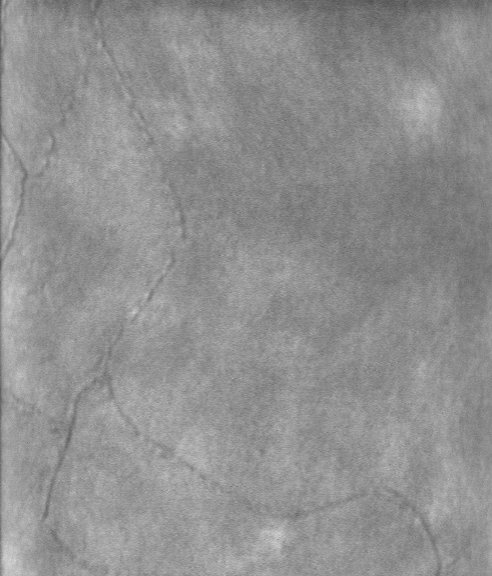
\includegraphics[scale=0.3]{Subject3_Session216_OD_(0,0)_1x1_980_OA790nm_dewarped_first.jpg}
		\caption{An image captured with AOSLO of a retinal capillary.}
		\label{fig:eye-capillary}
	\end{subfigure}
	\hfill
	\centering
	\begin{subfigure}[t]{0.45\textwidth}
		\centering
		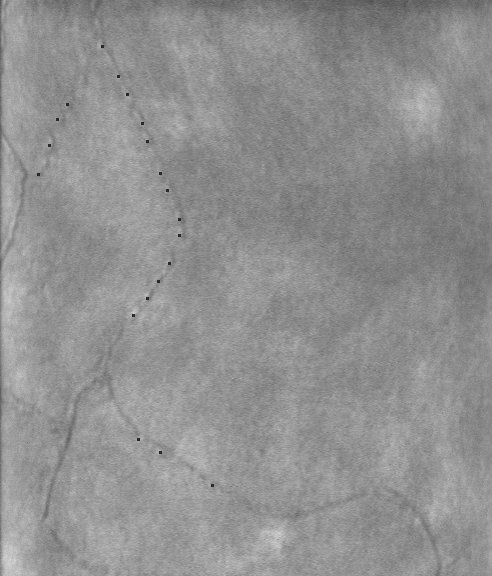
\includegraphics[scale=0.3]{Subject3_Session216_OD_(0,0)_1x1_980_OA790nm_marked_first.jpg}
		\caption{The same image with the blood cells marked}
		\label{fig:eye-capillary-marked}
	\end{subfigure}
	\vfill
	\centering
	\begin{subfigure}[t]{\textwidth}
		\centering
		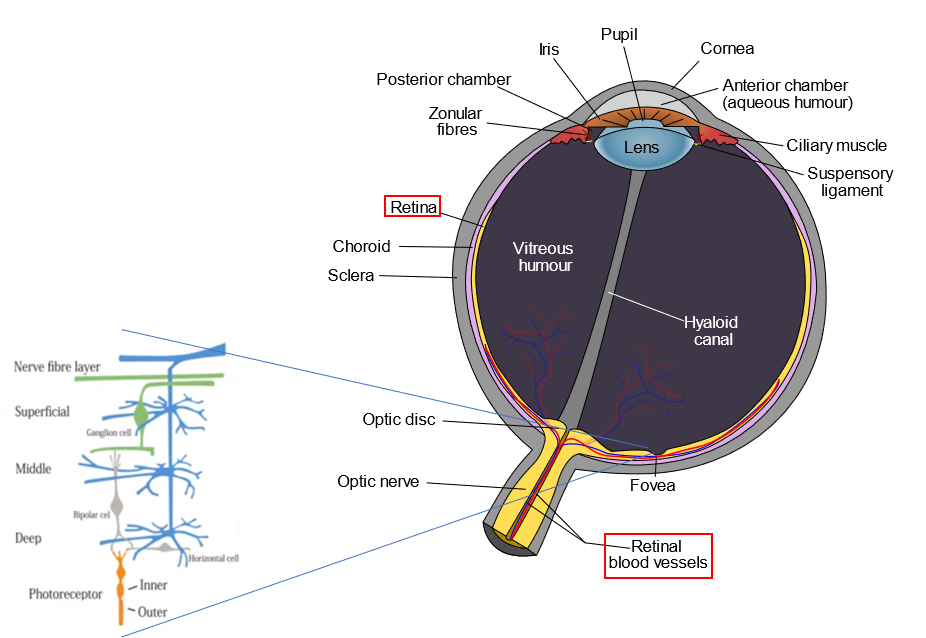
\includegraphics[width=\textwidth]{eye_anatomy.png}
		\caption{A picture of the eye anatomy\cite{eye_anatomy}.}
		\label{fig:eye-anatomy}
	\end{subfigure}
	\caption{\ref{fig:eye-capillary} \ref{fig:eye-capillary-marked} A still frame of a raster image captured using the AOSLO technique described in \cite{castro_rapid_2016}.
		The depth of field captures the red blood cells as they move in the capillaries in middle to deep levels of the retina as seen in \ref{fig:eye-anatomy}.
		The frame is a part of a bigger video found in this media link: \href{https://youtu.be/-7ew5sqOaTo}{(media)}.
	\ref{fig:eye-anatomy} The arteries and veins are fed through the optical nerve.
	In the image on the left\cite{noauthor_varying_nodate} we see that the retina hosts
	small vessels at many levels. }
	\label{fig:own-retinal-capillaries}
\end{figure}

Our group build a system based on the work in \cite{castro_rapid_2016}.
The Rapid high resolution image with dual-channel scanning technique uses Adaptive Optics Laser Opthalmoscope to produce two images of the same area in the retina with a very small time displacement.
Producing a single video of the capillaries with one channel captured at a frame of rate 32fps is not
enough because the time disparity between the two frames is too large and the correspondence of the frames can not be established.
This aliasing effect is demonstrated in Fig \ref{fig:aliasing-effect}.

\begin{figure}[ht]
	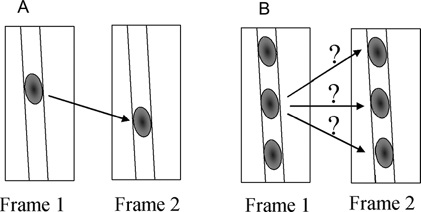
\includegraphics[width=\textwidth]{aliasing-effect.jpg}
	\caption{Image demonstrating aliasing effects from\cite{japee_automated_2005}. =
		 The red blood cells are abundant in the capillaries and they move fast.
	     As seen in B If the frame rate is not fast enough the time difference between the 
     	 between the frames is large so that it's impossible to establish a correspondence 
     	 between the cells in two consecutive frames.}
	\label{fig:aliasing-effect}
\end{figure}

To overcome this problem, the work in \cite{castro_rapid_2016} proposes a new technique where two different slightly different imaging wavelength are used at the same time.
As a result, two rasters of the same retina area are produced with a very small time disparity
that makes it possible to establish a correspondence.
The two images produces are called channels of the same image since they correspond to the same
retinal area but with a small temporal difference.
The time difference in \cite{castro_rapid_2016} is  4.7 ms while the implementation of our team
currently achieves 5.3ms due to differences between our scanners and the device used in the paper.
Another advantage of this technique is that this is a configurable value and may change over time.
The results of the images in the two channels can be seen in Fig \ref{fig:corresponding-channels}.

\begin{figure}[ht]
	\centering
	\begin{subfigure}[b]{.4\textwidth}
		\centering
		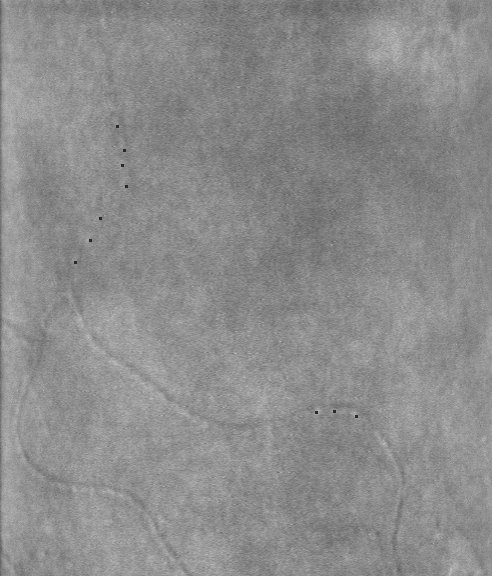
\includegraphics[width=0.75\textwidth, scale=0.75]{Subject3_Session216_OD_(0,0)_1x1_980_OA850nm_marked.jpg}
		\caption{Own image, channel 1 (790nm wavelength)}
		\label{fig:own-channel-a}
	\end{subfigure}
	\hfill
	\centering
	\begin{subfigure}[b]{.4\textwidth}
		\centering
		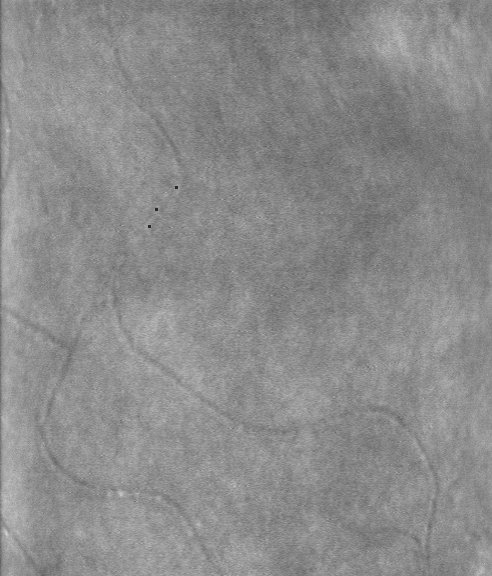
\includegraphics[width=0.75\textwidth, scale=0.75]{Subject3_Session216_OD_(0,0)_1x1_980_OA850nm_marked_corresponding_image.jpg}
		\caption{Own image, channel 2 (850nm wavelength)}
		\label{fig:own-channel-b}
	\end{subfigure}
	\vfill
	\centering
	\begin{subfigure}[t]{.4\textwidth}
		\centering
		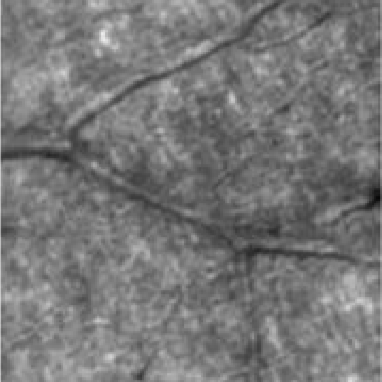
\includegraphics[width=0.75\textwidth, scale=0.75]{de_castro_channel_1.png}
		\caption{Image from \cite{castro_rapid_2016}, channel 1}
		\label{fig:de-castro-channel-a}
	\end{subfigure}
	\hfill
	\centering
	\begin{subfigure}[t]{0.4\textwidth}
		\centering
		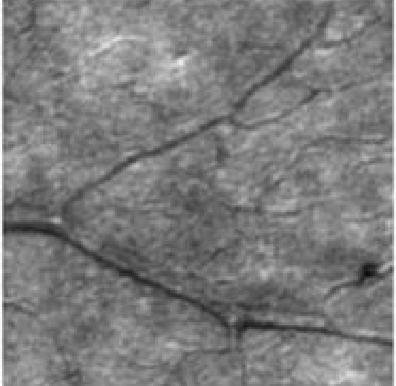
\includegraphics[width=0.75\textwidth, scale=0.75]{de_castro_channel_2.png}
		\caption{Image from \cite{castro_rapid_2016}, channel 2}
		\label{fig:de-castro-channel-b}
	\end{subfigure}
	\caption{The corresponding images of the same area in the retina captured by two imaging
		wavelengths for our own data \ref{fig:own-channel-a}\ref{fig:own-channel-b} and \ref{fig:de-castro-channel-a}\ref{fig:de-castro-channel-b}.
		It's obvious that the images from the two channels are not only temporally offset but
		spatially offset as well.
		This is because the imaging technique that is used to produce the time displacement between the channel also introduces some spatial offset which is known as seen in Fig \ref{fig:speed-of-cell-over-time}.
		The spatial offset is mostly constant and changes slowly as the video progresses and 
		can be easily fixed. 
	}
	\label{fig:corresponding-channels}
\end{figure}

In the same paper they also describe a method for measuring the velocity of the erythrocytes by using post-processing techniques.
To do this they firstly try to detect the cells by first normalizing the frames of the video for each channel and then they thresholded the images to create a binary image of each frame.
The threshold is N times the standard deviation of the pixel intensity over the all the frames 
of the video.
Then by applying a morphological open operator to the binary images they get a set of location of the cells.
Instead of comparing the cell locations directly between the channels they advise for creating an ``average cell image'' by averaging all the cells for each frame.
By measuring the displacement of the ``average cell images'' between the two channels the average red blood cell can be extracted\ref{fig:castro-average-cell}.

\begin{figure}[ht]
 	\centering
 	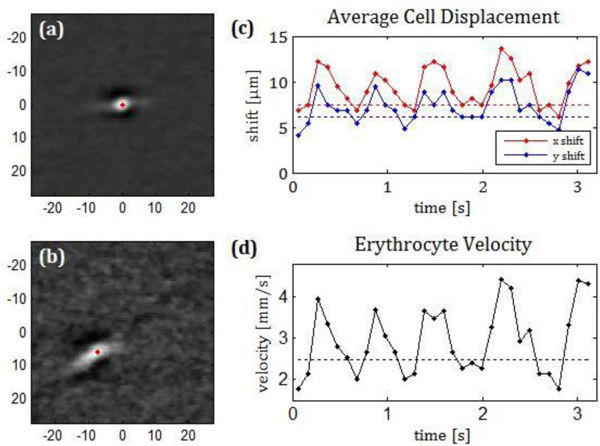
\includegraphics[width=0.5\textheight]{castro-average-cell.png}
 	\caption{Figure from \cite{castro_rapid_2016}.
 		In (a) we see the average cell created from the first channel and in
 		in (b) the corresponding average cell for the second channel that is 4.7 ms ahead
 		of the first . By measuring the 
 		x and y displacement(c) the average red blood velocity(d) can be extracted}.
 	 	We want to follow a similar process as shown in Fig \ref{fig:speed-of-cell-over-time}.
 	\label{fig:castro-average-cell}
\end{figure}


This method allows for measuring a bigger range of retinal capillary velocity than was previously possible as shown in the results from high frame rate fundus illumination system \cite{bedggood_direct_2012}, or on leukocytes using either the entoptic phenomenon \cite{riva_blue_1980}\cite{grunwald_effect_1993}, or other single channel imaging techniques with AOSLO \cite{martin_pulsatility_2009}\cite{martin_direct_2005}\cite{tam_speed_2011}\cite{tam_characterization_2011} as reported in \cite{castro_rapid_2016}.
The method in\cite{castro_rapid_2016} can measure velocities higher than was previously possible with the methods described before because red blood cells can be faster than white blood cells due to their
size. 
It also produces comparable results to labeling with fluorescein\cite{yang_fluorescent_1997}\cite{paques_evaluation_2000} which are invasive methods.
Additionally, this method is better for smaller vessels  while other techniques such as \cite{zhong_vivo_2008} or \cite{riva_laser_1972} are better for larger vessels.
One additional benefit of this method is that it allows for a bigger area of the retina to be image.
The benefit is twofold because we can  study a bigger retina area and also artifacts from eye movement can be corrected more easily using techniques such as \cite{dubra_registration_2010}.

Our team implement the same setup in \cite{castro_rapid_2016} but unfortunately the image processing pipeline to track the blood cells did not work for our case since, due to differences in the implementation, the cells from our setup lack the bright characteristic that is present in the cells in \cite{castro_rapid_2016}. 

For this reason it was decided to research into other potential methods for identifying the red blood cells in our images.
In this light, we review the work done in image recognition of conic photo-receptors captured using AOSLO techniques.
The conic shape and structure of the images of the phototoreceptors\ref{fig:bergelles-photoreceptors} is different from our images but since the rasters were generated using AOSLO techniques, they serve as good candidates for potentially similar implementations for our problem of image recognition of erythrocytes.

\begin{figure}[ht]
	\centering
	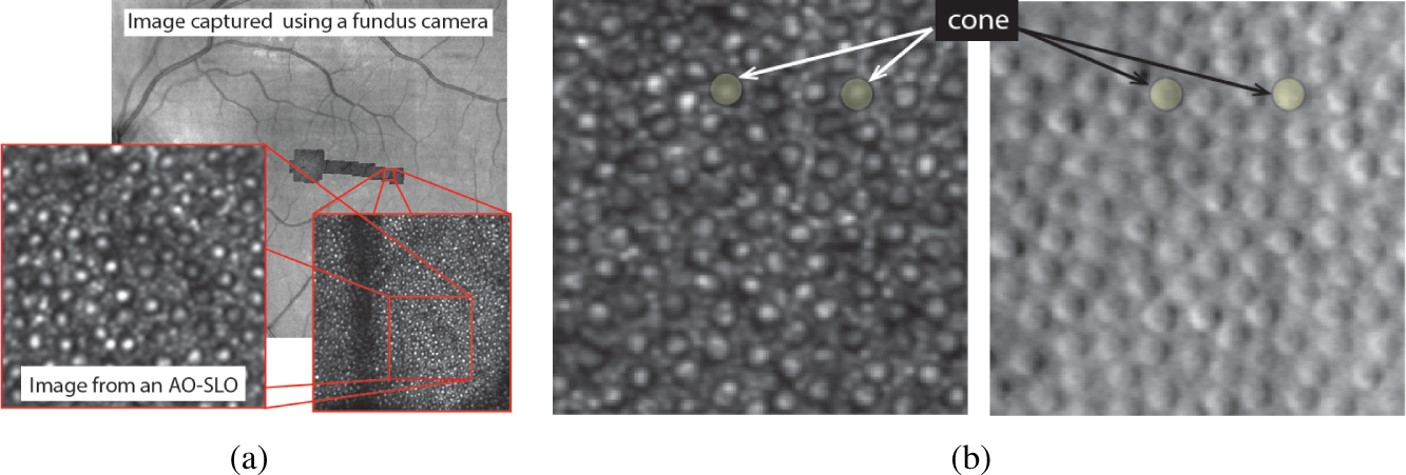
\includegraphics[width=\textwidth]{bergelles-photoreceptord.jpg}
	\caption{Figure of photoreceptors rasters from \cite{bergeles_unsupervised_2017}.
		In (b) we see images captured with two different AOSLO techniques.
	}
	\label{fig:bergelles-photoreceptors}
\end{figure}

One implementation we are going to review is \cite{bergeles_unsupervised_2017}. 
The paper presents a way to classify the conic photoreceptors that lie in the same area of the retina captured using AOSLO but at a different depth of field range.
To classify and detect the photoreceptors they present an image processing pipeline that uses SVN.
In brief, the pipeline includes the photoreceptor's size is estimation using an automated process (Yellott's ring\cite{cunefare_automatic_2016} \cite{cooper_automatic_2013}) or manually, use of bilateral and a Gaussian filter, adaptive histogram equalization, adaptive sliding-window enhancement is applied to enchance the contrast between the left/dark and right/bright sides of the cones, aggressive thresholding to create a binary image, non-overlapping extremal region detection to detect the centroids, a preliminary model for cone extraction and finally a model for refinement and cone detection using a Support Vector Machine (SVM). 
The process is described in great detail in the paper.
There are 11 configurable hyperparameters and some of them can be semi-automatically be set based on heuristics.
The results reported in the paper show that the model is precise and it's results are comparable to a human grader for images of healthy retinas and have a positive precision and recall on images of retinas with Stargardt disease.
It's also reported that the model can outperform the, at the time, state of the art model developed in\cite{cunefare_automatic_2016}.

Although the model shows promising results, it might not be the best choice for red blood detection in our images. 
The method creates a cone-model that accounts for the characteristic shape and intensity of the photoreceptor cells.
In addition, the model is dependent on the spatial arrangement of the photoreceptor mosaic. 
As a result, when the model is presented with images of the photoreceptor mosaic of people with Stargard disease, which is more sparse, it's performance drops and both the precision and recall of the model are significantly lower.
For this reason, the parameter configurations and control will most likely not work for our problem, since our erythrocyte images not only have a different shape, they also have a different structure.

Hence, it was decided to follow a different paradigm of image classification, one that was shown to outperform traditional machine learning techniques\todo{add citations} and that is to use deep learning for image classification.
Deep networks learn features directly from the data and do not rely to ad-hoc rules
that are unique to the data-set.
As a result, such networks are more adaptable.
This is more appealing for our case because deep learning models can be
generic and a model that is a trained for a particular data-set can be
adapted and be used for other data-set.
One drawback of deep learning is that it can be outperformed from traditional machine learning techniques when the the amount of training data is little.
This can be sometimes circumvented with techniques such as data augmentation\cite{perez_effectiveness_2017} which was shown to work with great success in the past\cite{ronneberger_u-net_2015}.
Deep Convolution Neural Networks (CNNs) \todo{cite } have been shown to work for different image analysis tasks in many fields including optical imaging\cite{gulshan_development_2016, perez_effectiveness_2017, li_cross-modality_2016, fu_retinal_2016, fang} with great performance.


For this reason we would like to review the methods described in \cite{cunefare_open_2017} and the later \cite{cunefare_deep_2018}.
Both of this methods try to classify and locate conic photoreceptors in
AOSLO images using image classification neural networks.
Because of reasons we talked before, we believe this work can be adapted for our use-case as well.
The implementation for cell detection and localization is not dependent on the structure and appearance of the cone cells but it is expected that the network should be adapted to work better with our own data.
Next, we would summarize the implementation that is described in the paper.
First images of the photoreceptor mosaic are generated from a random sample of people and experts mark the centers of each photoreceptor.
To create a training set for the binary classifier we need images for cone and non-cone cells.
A window of a fixed size is drawn around the marked centers to extract patches of cones.
To produce images of negatives a voronoi pattern is created around the centers.
Then random points from the edges of the voronoi pattern are selected as centers for the 
non-cone patches.
This process is also demonstrated in Fig\ref{fig:cunefare-training-data-generation}.

\begin{figure}[h]
	\centering
	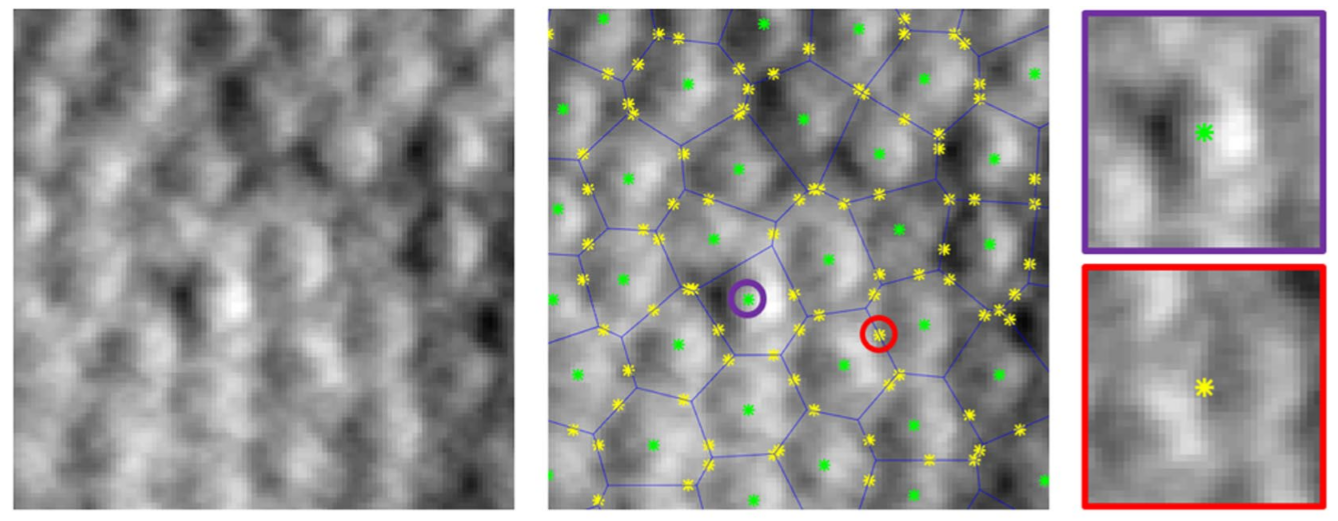
\includegraphics[width=\textwidth]{cunefare_generating_data.png}
	\caption{Image from \cite{cunefare_open_2017}. Shows the training data generation process for the classification CNN training. (a) The original image of the 
	photoreceptor mosaic, (b) Image (a) with the center of the photoreceptors marked by
    an expert and a voronoi diagram around them. Points on the voronoi edges are randomly
    selected as centers of non-photoreceptor (negatives) patches. 
    (c) An example of a cone (top) and non-cone (bottom) patch extracted from the marked image (b).  }
	\label{fig:cunefare-training-data-generation}
\end{figure}


Once the training set is created the CNN classifier can be trained to detect cone from non-cone images.
The CNN described in\cite{cunefare_open_2017} is a modification of the famous AlexNet\cite{krizhevsky_imagenet_2012}.
It consists of Convolutional layers to generate feature maps, pooling layers which are known to improve computational performance and increase invariance to small distortions\cite{jarrett_what_2009},
Rectified linear units (ReLU) activation layers to introduce non-linearities\cite{jarrett_what_2009},
batch normalization layers which is reported to increase training speed and reduce overfitting by normalizing layer inputs using their mean statistic\cite{ioffe_batch_2015}.
In the end there are fully connected  layers, again with ReLU activations, for the classification part.
The last layer has two outputs and is fed to a soft-max layer to provide a probability distribution for cone and non-cone\cite{bishop_pattern_recognition_2006}.
\todo{add references}
With the model defined the weights for the convolution and fully connected layers must be trained.
Each iteration, also called an epoch, a subset of the training set, called a mini-batch, is fed to the network.
For each image in the mini-batch a label is predicted with a probability distribution from the soft-max layer, i.e 75 per cent cone and 25 per cent non-cone.
In the training process, because the label is known for each image, 
a loss function measures the distance of the predicted output and the actual label.

Proportionally to this distance, the network adjusts the weights, with a process called back propagation.
This whole training process is called gradient descent because during the forward pass a gradient is calculated 
for each weight with the goal to minimize the loss function.

With sufficient training data the network can potentially classify cones from non-cones with a high accuracy.
It's good to mention here that part of the data-set should be just for testing the performance of the classifier and should not be used for the training process.
The photoreceptors must then be localized in the image.
In \cite{cunefare_open_2017}, a patch is created around each pixel of the image and all the patches are classified
with the trained CNN.
The result is a gray-scale image with the probability of each pixel being the center of a cone.
Next, a Gaussian smoothing is applied on the probability map followed by an extended-maxima transform.
The resulting binary image is thresholded.
Finally, the center of the remaining clusters is considered to be the center of the cone.
For additional information for the threshold values please see \cite{cunefare_open_2017}.

The results are compared against the gold standard for detecting photoreceptors that uses graph theory and dynamic programming (GTDP)\todo{cite} and a previous work
that we mentioned earlier that uses adaptive filtering and local detection (AFLD) \cite{cunefare_automatic_2016}.
In both cases the  results are very comparable with a true positive rate ranging 0.943 to 0.989 and a false discovery rate of 0.034 and as low as 0.003.
For a more detailed description of the evaluation method please refer to\cite{cunefare_open_2017}.

The results are very appealing since it shows that the model can compete with state of the art methods.
Contrary to the other techniques, it has the advantage that it can be adapted for applications with different modalities since it uses a CIFAR network modification that can be trained for different data-sets .
The GTDP and AFLD models were created with assumptions and rules that are specific for the 
photoreceptor mosaic.
The software for  model in\cite{cunefare_automatic_2016} is open source and is shared by the authors.
Furthermore, they encourage the use of software for testing and adapting it to new training data sets and imaging conditions.

Image classification using CNNs can potentially solve the problem of locating the red blood cells in our videos.
Once the red blood cells are located correspondence must be made between the two channels of the frame to measure the velocity.
An alternative is to use the method used in\cite{castro_rapid_2016} with the calculation 
of the ``average cell"\ref{fig:castro-average-cell}.
Because this method creates ``average cell" for the two channels by adding all the detected
cells it is required for the cells to move in the same direction. 
For example, if we take the mean of two erythrocytes that move in opposite directions then their ``average cell" image will be in the same position and the speed would be 0.
The solution in\cite{castro_rapid_2016} is to manually select a small capillary segment.
This could be also implemented for our case since in a single video from a patient 
the capillary structure is guaranteed to stay the same.
Since a fully automatic tool for measuring the blood velocity, it is useful
to research on existing methods for blood vessel segmentation.
By having a capillary segmentation the benefit is threefold,
The search-space for potential blood cells would be drastically reduced since
most of the image consists of non-cells making the localization of the cells more efficient.
In addition, the training set should contain more meaningful non-cell images than simply empty patches, increasing the performance of the classifier and potentially reducing false positives.
Finally, if the capillary segmentation is known then we could analyze a
small segment of it at a time so that it's guaranteed that the blood cells move 
in the same direction.

Currently, there is a growing literature for blood vessel segmentation 
in retinal images\cite{liskowski_segmenting_2016}\cite{fu_retinal_2016}\cite{li_cross-modality_2016}. 
However, the data-set for this problems focuses on fundus imaging\cite{fraz_blood_2012} and is focused on bigger blood vessels in the 
retina (arteries and veins) and not on capillary. 
Additionally, fundus imaging is very different and produces images with very different features than the ones we produce.
As previously stated we could potentially adapt an existing deep learning techniques for our use-case.
One promising such segmentation network is DeepVessel\cite{fu_deepvessel_2016} which produces state of the art results.
To train for segmentation using a supervised machine learning method it is required to have a ground truth for the capillaries which we currently don't
have.
We could produce ground truth  for some of our images but with that we could still
have a little amount of data.
Data augmentation techniques could be used to decrease the amount of data needed.
Moreover, transfer learning is shown to work\cite{jiang_retinal_2018} when 
there is a lack of labeled data available.
With transfer learning, we could potentially train a neural network like
DeepVessel with publicly available fundus images and then retrain part of 
the network with images from our training data.


\section{Proposed Method} 
In this section we propose a method that uses some of the techniques that were mentioned before.

The end-goal of this thesis is to create a tool that takes a video of the retina
captured with AOSLO and produces statistics about the velocity of the blood flow 
based on tracking the erythrocytes moving in the capillaries.
As mentioned before, the method 
Ideally, we would like the process to be automatic but in case not all components
of the system are implemented due to time constraints the user should be able
to mark areas with capillaries.

The process of tracking and measuring the blood cells can be broken down to three 
big steps.
First the locations of the blood cells must be located in both channels for each frame of the video.
Next, the correspondence between the cells must be established.
Finally, since we know the time disparity between the two channels we can measure the average velocity of the blood flow\ref{fig:speed-of-cell-over-time}.

\begin{figure}[ht]
	\centering
	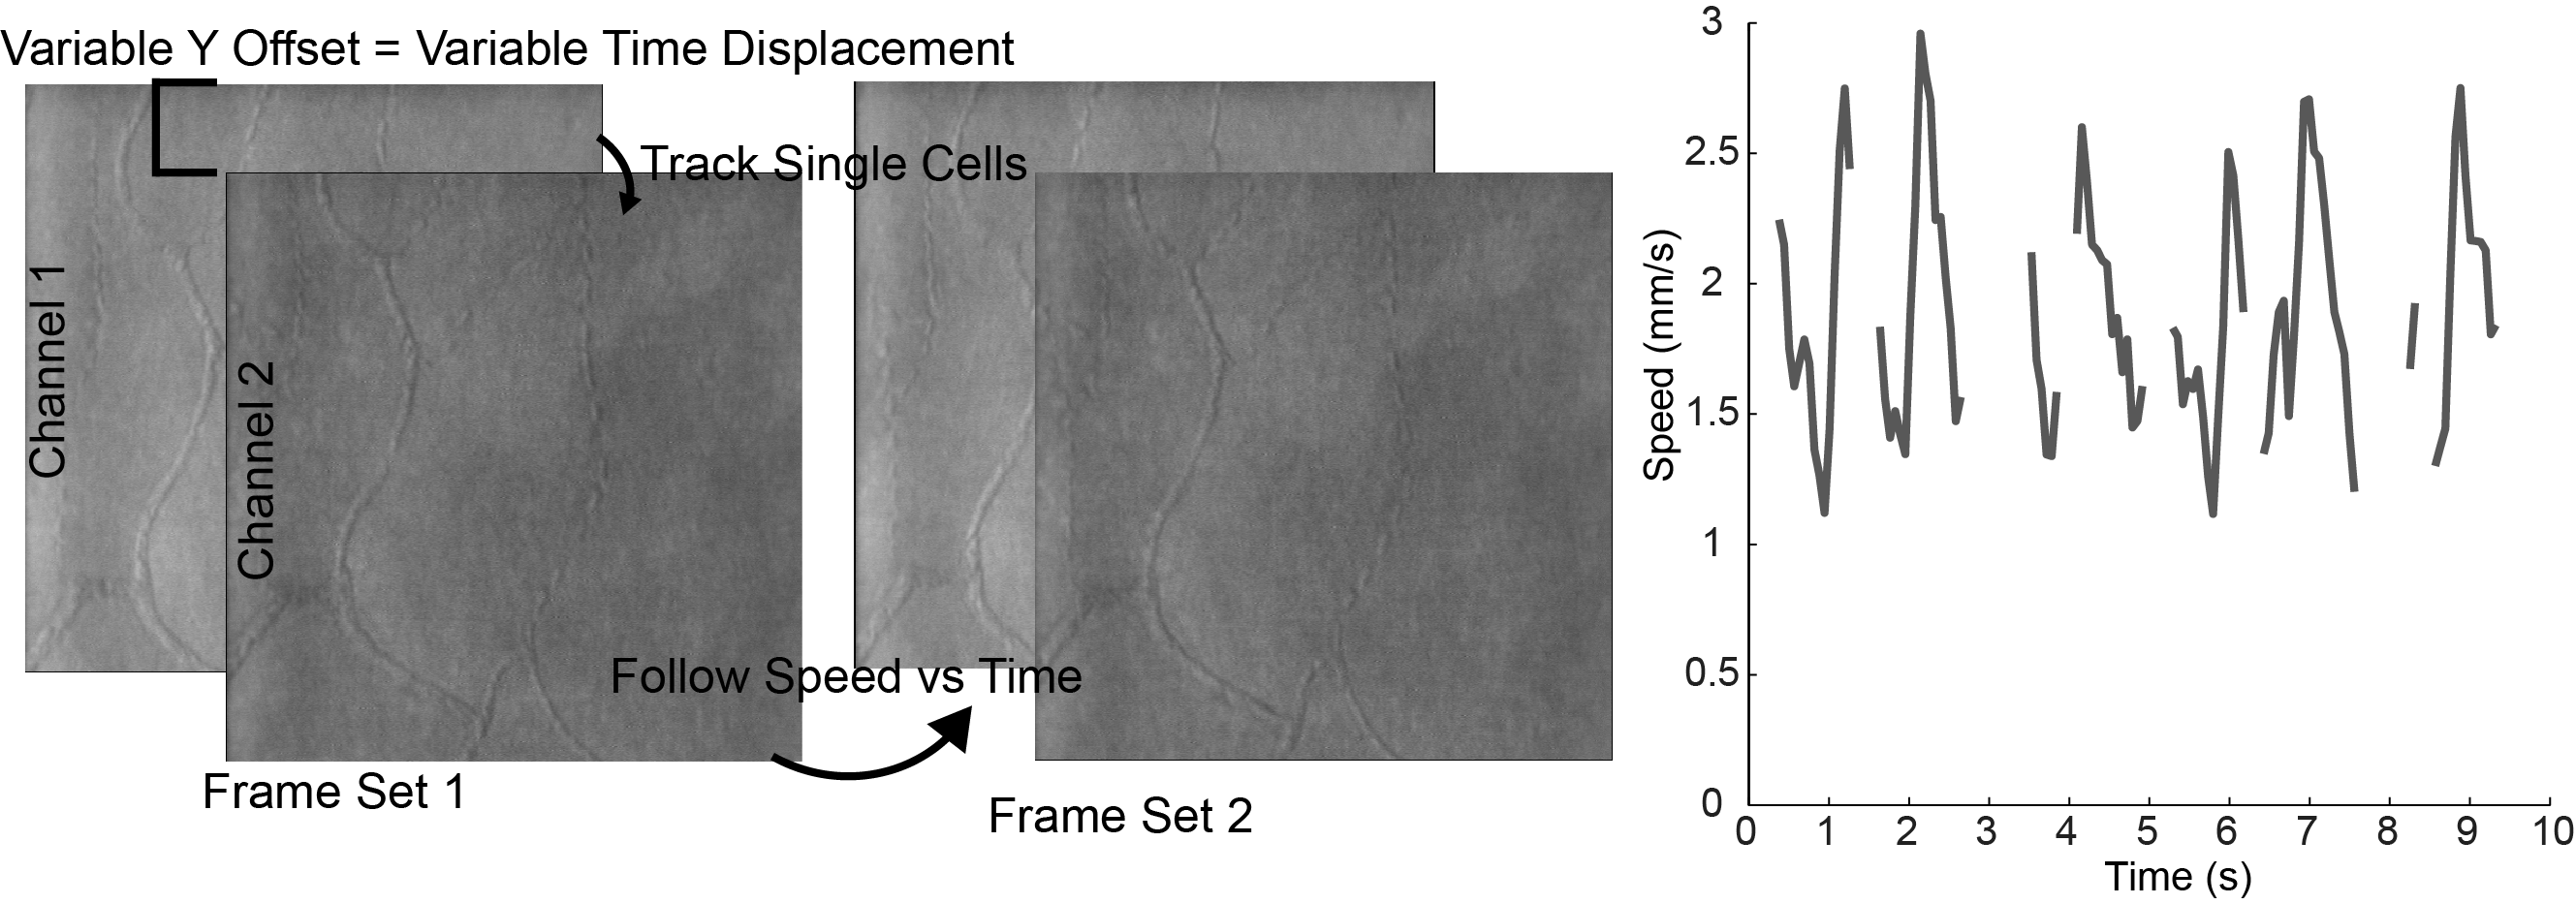
\includegraphics[width=\textwidth]{spatial_offset.png}
	\caption{Measuring the speed of a red blood cell over time.}
	\label{fig:speed-of-cell-over-time}
\end{figure}

For the first part, we decided to follow the work done in \cite{cunefare_open_2017}.
The process to localize the erythrocytes will be similar to what was described 
in previous section.
In brief, the training set for the cell and no-cell images should be created by 
extracting a fixed window patches around cell and no-cell points\ref{fig:own-data-blood-cells}.
The cell locations are marked by an expert in some of the frames and the no-cell
locations are to be extracted with the voronoi pattern with the method described
in\cite{cunefare_open_2017}.

\begin{figure}[ht]
	\centering
	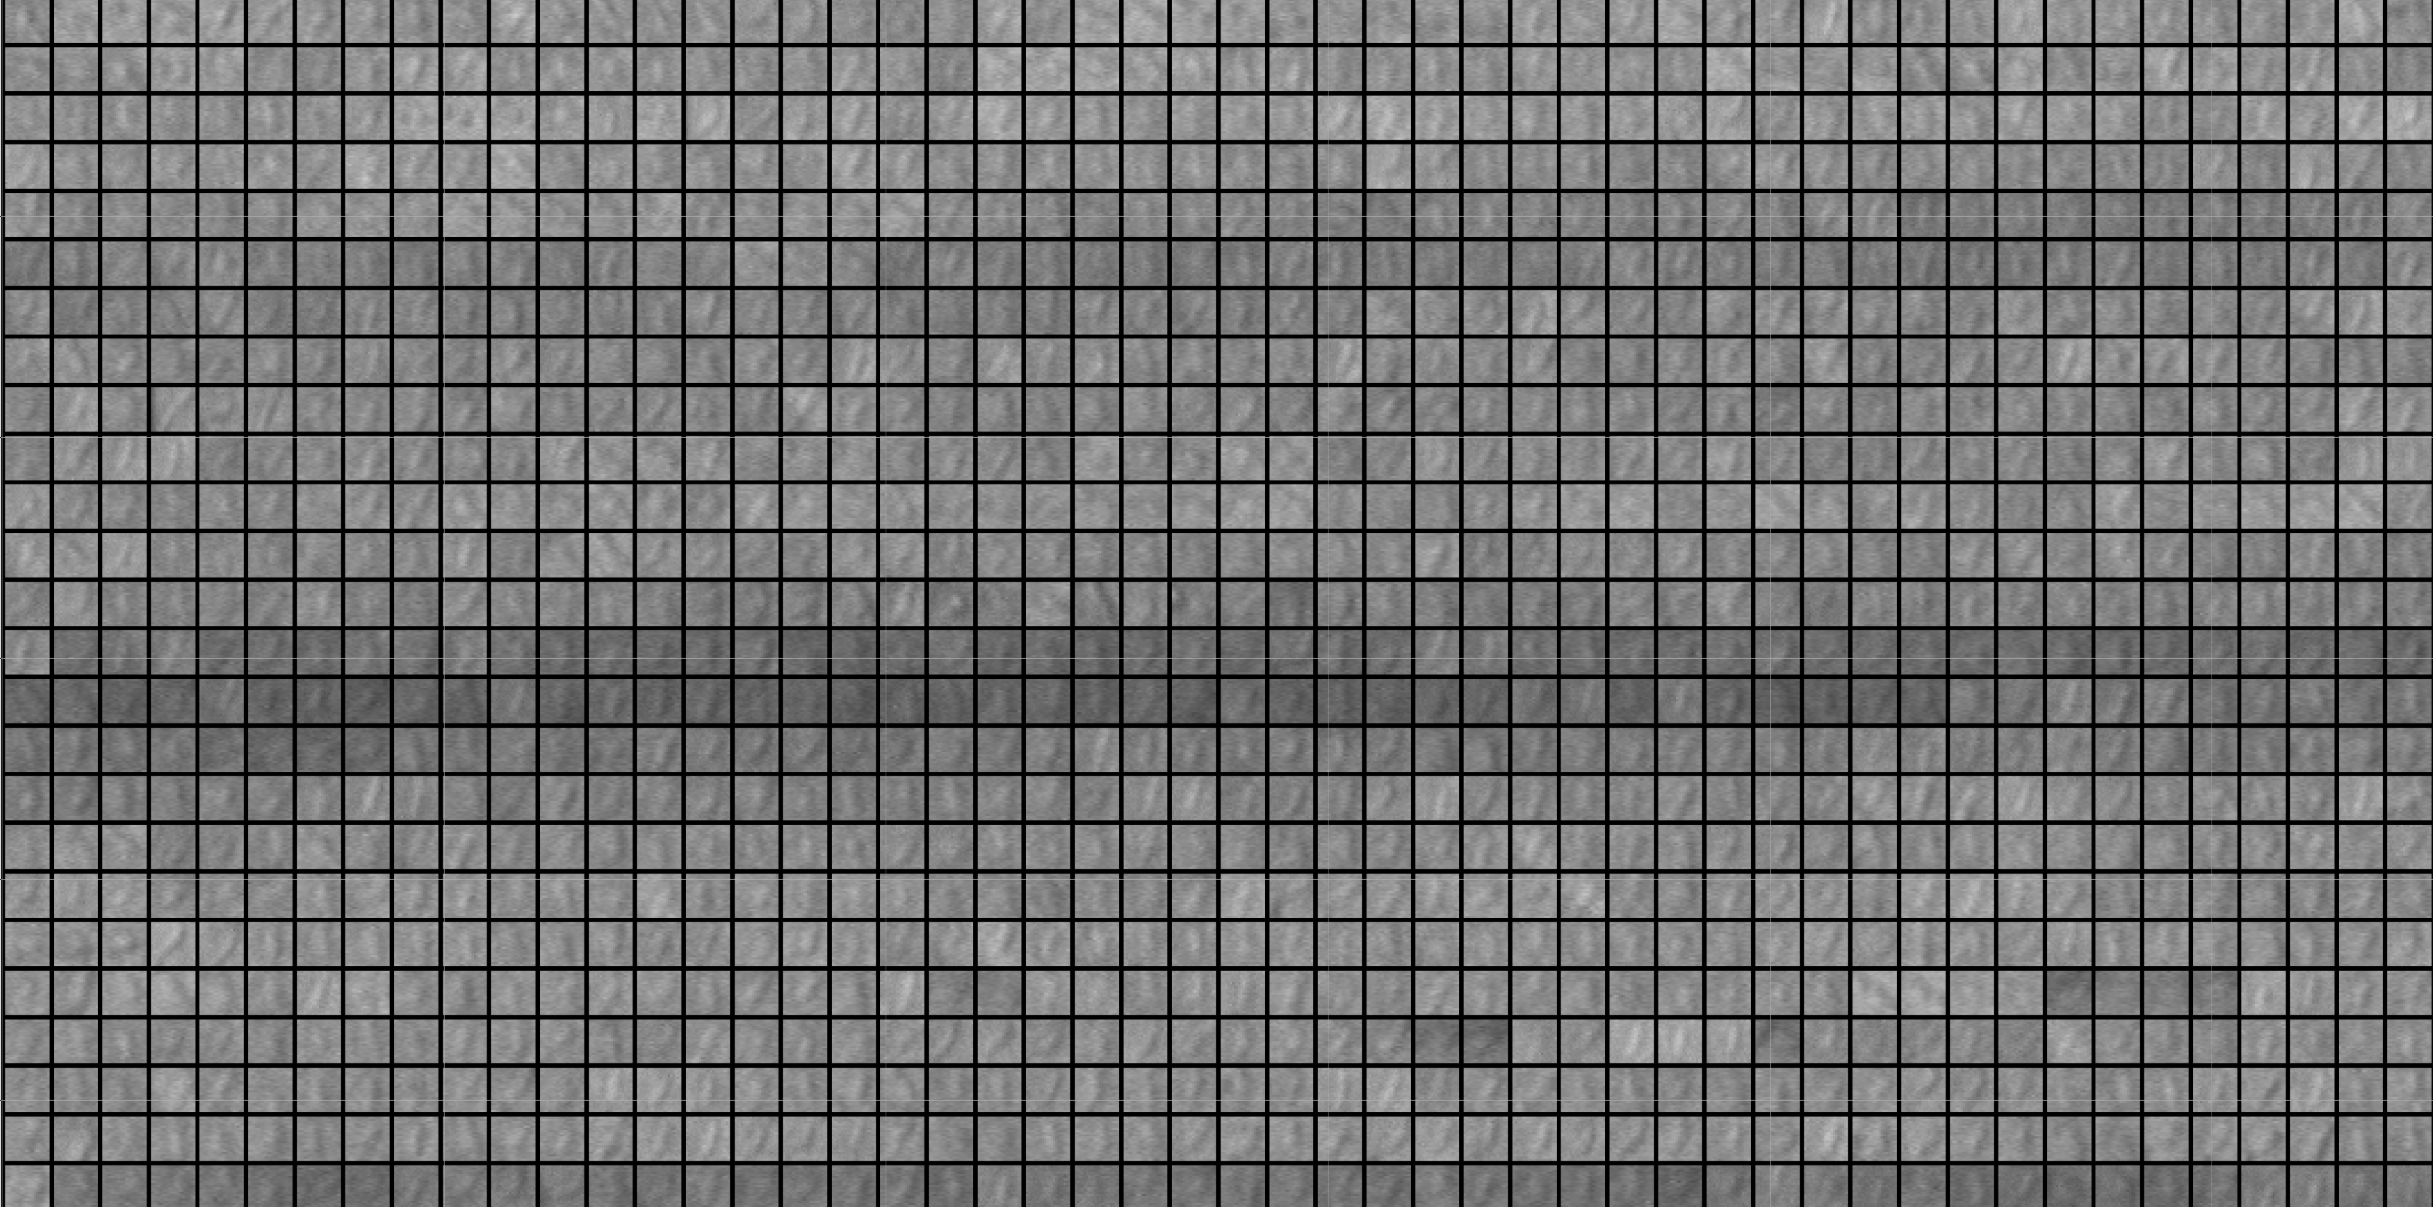
\includegraphics[width=\textwidth]{extracting_data_own.png}
	\caption{Red blood cell patches extracted from \href{https://youtu.be/-7ew5sqOaTo}{(media)}. }
	\label{fig:own-data-blood-cells}
\end{figure}

Then a AlexNet\cite{krizhevsky_imagenet_2012}-like CNN should be trained until the desired performance is achieved.
A potential challenge for this stage would be the lack of sufficient data quantity.
To circumvent this data augmentation could be used.
The red blood cell patches seem to have similar size and intensities so we believe that it could possible to augment our data-set with fake images by transforming existing ones.
Another likely problem that could arise is overfitting to the training data.
Because the retina of different subjects can have different reflective properties, and the conditions of the recording session are also different from
person to person it's very likely that the network will fail when presented with
new and unseen images that are dissimilar to the the training data.
To get around this problem, regularization techniques can be applied such as dropout layers, early stopping, L2 \& L1 regularization\cite{Goodfellow-et-al-2016} or, again, with data augmentation\cite{Goodfellow-et-al-2016} . 

Assuming a classifier with good performance is achieved, the next step is to 
locate the cells.
Firstly, a patch should be extracted around every pixel. Each patch should be 
fed through the classifier.
Just like in \cite{cunefare_open_2017} the resulting probability map should be then be smoothed and extended-maxima transform must be applied.
After weak candidates should be filtered.
The centers of the remaining clusters is the predicted location of the cells.

For the next step, instead of directly establishing correspondence,
it was decided the ``average cell" technique from\cite{castro_rapid_2016}
should be implemented.
As previously mentioned, the blood cells should move in the same direction in
the segment of the capillary or else the estimated velocity is wrong.
For this part, the segment 

\begin{figure}[ht]
	\centering
	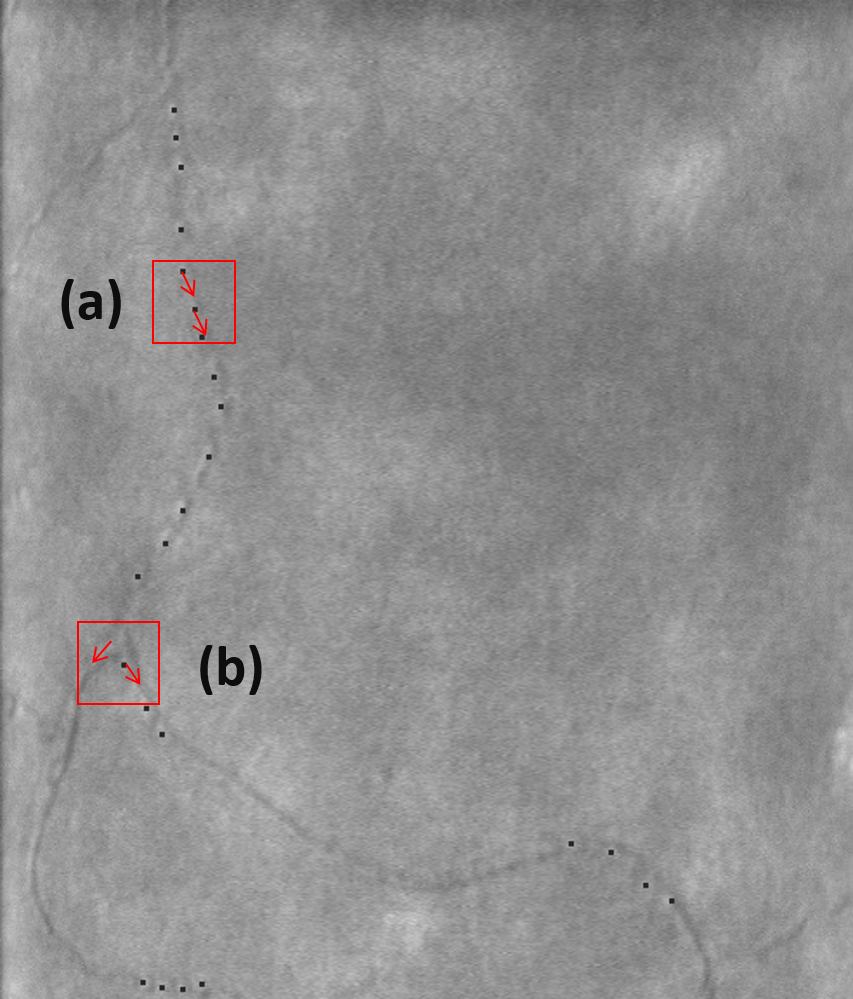
\includegraphics[width=\textwidth]{segment-example.png}
	\caption{caption}
	\label{fig:labep
\end{figure}


\section{Proposed Evaluation}


\end{document}
